\documentclass[11pt]{article}
\usepackage[margin=1.0in]{geometry}
\usepackage{tikz}
\usetikzlibrary{positioning, arrows.meta, fit, backgrounds}
\usepackage{amsmath}
\usepackage{xcolor}
\usepackage{hyperref}
\hypersetup{colorlinks=true, linkcolor=blue!50!black, urlcolor=blue!50!black,
  citecolor=blue!50!black}

\newcommand{\code}[1]{\texttt{#1}}
\newcommand{\file}[1]{\texttt{\small #1}}
\sloppy

\title{Scaling the ``multi-sim'' depo fan-out\\
  \large WCT TbbFlow fan multiplicity and the DUNE FD-VD}
\author{Brett Viren\thanks{Draft analysis prepared with AI (Claude) assistance;
  claims, figures and recommendations are to be reviewed before acting.}}
\date{2026-10-19}

\begin{document}
\maketitle

\begin{abstract}
The dune10kt-vd WC/LS ``multi-sim'' job fans a drifted depo set out to one
processing ``finger'' per TPC.  The fan is built as a single \code{DepoSetFanout}
whose output multiplicity equals the number of TPCs.  The Wire-Cell Toolkit
(WCT) TbbFlow layer caps a single fan at multiplicity~10, so the job aborts once
more than ten TPCs are requested --- well short of the DUNE far-detector vertical
drift (FD-VD), which has of order 320 charge-readout units (CRUs).  This note
locates the limit precisely (it now lives in WCT, not in oneTBB), documents the
layered ``fan-of-fans'' machinery that \emph{already exists} and is already used
to reach~320 in the ``full'' mode, and analyses the space of fixes.  It critiques
the two approaches most readily reached for --- a Jsonnet fan-of-fans abstraction,
and extending the enumerated C++ fan sizes --- and compares them with
\code{broadcast\_node}-based unbounded fan-out, bounded auto-enumeration, a
runtime distributor, and simply not building a wide fan.  The recommendation is
layered: adopt the existing \code{multifanout} tree in the multi-sim path now
(zero C++ change, already proven), add a small auto-layering helper to remove its
ergonomic sharp edges, and reserve a C++ \code{broadcast\_node} fan-out for the
case where a genuinely flat, unbounded fan is wanted.
\end{abstract}

\tableofcontents

\section{Problem}

The ``multi-sim'' modal layer
(\file{dune10kt-vd/wcls-sim-drift-simchannel-nf-sp-multi.jsonnet}) builds one
self-terminating finger per TPC and joins them with a single fan-out sink:

\begin{verbatim}
    local fanout = g.fan.sink('DepoSetFanout', fingers, 'multi_sim_fanout');
\end{verbatim}

\noindent
\code{g.fan.sink} (\file{cfg/pgraph.jsonnet}) emits one \code{DepoSetFanout}
whose \code{multiplicity} is \code{std.length(pipelines)}, i.e.\ the number of
fingers:

\begin{verbatim}
    sink :: function(fout, pipelines, name="fansink", tag_rules=[]) {
        local fanmult = std.length(pipelines),
        local fanout = $.pnode({ type: fout, ...
            data: { multiplicity: fanmult, ... }}, nin=1, nout=fanmult),
        ...
\end{verbatim}

\noindent
With $N_{\mathrm{TPC}}\le 4$ (the demo) this is a 4-way fan and works.  For the
FD-VD the physical target is $N_{\mathrm{TPC}}\sim 320$.  A single 320-way
\code{DepoSetFanout} cannot be realised: the TbbFlow fan wrappers hard-assert a
maximum multiplicity of~10 (\S\ref{sec:background}), so the job aborts at
construction.

\section{Where the limit actually lives}
\label{sec:background}

\subsection{WCT's compile-time tuple fan}

A WCT \code{IFanout} node is realised in TbbFlow by \code{FanoutWrapper}
(\file{tbb/inc/WireCellTbb/FanoutCat.h}).  The run-time output multiplicity is
translated to a compile-time template parameter by an exhaustive
\code{if}-ladder, guarded by an assertion:

\begin{verbatim}
    int nout = wcnode->output_types().size();
    Assert(nout > 0 && nout <= 10);   // fixme: exception instead?
    if (1 == nout)  m_sender_ports = build_fanouter<1>(...);
    ...
    if (10 == nout) m_sender_ports = build_fanouter<10>(...);
\end{verbatim}

\noindent
\code{build\_fanouter<N>} instantiates a TBB \code{split\_node<TupleType>} where
\code{TupleType} is \code{type\_repeater<N,msg\_t>::type} --- a tuple of $N$
identical \code{msg\_t} ports --- plus a per-port sequencer (\code{seq\_node}) to
restore ordering after the split node's unlimited concurrency.  \code{FaninCat.h}
is the mirror image: \code{FaninWrapper} asserts \code{nin <= 10} and selects
\code{build\_faniner<1..10>}, each instantiating a \code{join\_node<TupleType>}.

Two facts follow:

\begin{enumerate}
\item \textbf{The cap is a WCT choice, not a TBB limit.}  As of oneTBB~2021 the
  \code{split\_node}/\code{join\_node} templates are fully variadic --- there is
  no intrinsic port-count ceiling (issue~\#236).  The ceiling of~10 is the length
  of WCT's hand-written \code{if}-ladder and the \code{Assert}.
\item \textbf{The real C++ constraint is runtime$\to$compile-time translation.}
  C++ has no way to turn a value held in a run-time variable into a template
  parameter other than writing code for every possible value.  So even with a
  variadic TBB, a WCT fan of run-time multiplicity $N$ still needs \emph{some}
  mechanism to reach the matching \code{build\_fanouter<N>} instantiation.  The
  variadic update removes the need to \emph{hand-write} each tuple type, not the
  need to \emph{enumerate} the instantiations.
\end{enumerate}

\subsection{Cost of large homogeneous tuples}

Issue~\#236 reports a micro-benchmark of instantiating large TBB fan tuples.
With $\sim$100 \emph{distinct} port types, compilation ballooned to
$\sim$30\,s and the object to $\sim$4.5\,MB; with 100 \emph{identical} types it
was $\sim$4.5\,s and $\sim$516\,kB.  WCT's fans are homogeneous
(\code{type\_repeater<N,msg\_t>}), so they sit in the cheaper regime --- but the
cost still grows with the largest instantiated $N$, and it is paid at every build
of the \code{tbb} package.  This is the quantitative argument against simply
pushing the enumerated ceiling very high.

\subsection{The target geometry}

The FD-VD motivating figure is $\sim$320 CRUs (issue~\#495).  The in-tree
example geometry \file{dunevd10kt\_3view\_30deg\_v6\_refactored\_1x8x14} realises
this scale; each CRU carries 1536 channels.  The ``multi-sim'' job wants one
independent per-CRU output product set, hence a fan as wide as the CRU count.

\section{What already exists: the layered ``fan-of-fans''}
\label{sec:existing}

The fan-of-fans tree the user proposes to ``write'' (candidate~S1,
\S\ref{sec:s1}) \emph{already exists} and is in production use.
\file{cfg/pgrapher/common/funcs.jsonnet} provides:

\begin{itemize}
\item \code{multifanpipe(fout, pipelines, fin, fout\_nnodes, fout\_multi,
  fin\_nnodes, fin\_multi, ...)} --- a fan-out tree, the pipelines, and a
  symmetric fan-in tree; and
\item \code{multifanout(fout, pipelines, fout\_nnodes, fout\_multi, ...)} --- the
  fan-out tree only, with self-terminating pipelines (a \emph{sink}).
\end{itemize}

\noindent
Each tree is described by two per-layer lists: \code{nnodes[i]} (the number of fan
nodes in layer $i$) and \code{multi[i]} (the out-multiplicity of each node in
layer $i$).  The docstring's own examples reach the FD-VD scale:

\begin{verbatim}
    // for dune-vd 1x8x14, one can choose nnodes=[1,8,16], multi=[8,2,7]
\end{verbatim}

\noindent
and the ``single/full'' modal layer
(\file{...-single.jsonnet}) already fans to 320 through a four-layer tree whose
largest single fan is~10:

\begin{verbatim}
    f.multifanpipe('DepoSetFanout', process_pipes, 'FrameFanin',
                   [1, 2, 8, 32], [2, 4, 4, 10],  // fan-out layers
                   [1, 2, 8, 32], [2, 4, 4, 10],  // fan-in  layers
                   ...)
\end{verbatim}

\noindent
Here the leaf count is $32\times10=320$ and every layer multiplicity
($2,4,4,10$) is $\le 10$, so every individual fan node is legal.  The tree depth
is~4.  \textbf{So the ``full'' mode already does at~320 exactly what the
``multi-sim'' mode fails to do at~$>$10} --- it simply uses \code{multifanpipe}
instead of the flat \code{g.fan.sink}.

\begin{figure}[h]
\centering
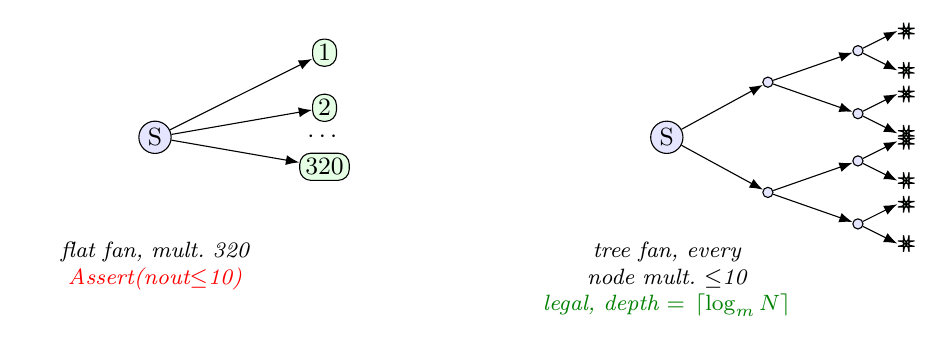
\begin{tikzpicture}[>=Latex, node distance=6mm and 10mm,
    every node/.style={font=\small},
    f/.style={draw, circle, inner sep=1.3pt, fill=blue!10},
    leaf/.style={draw, rectangle, rounded corners, inner sep=2pt, fill=green!10}]
  % flat (illegal) fan
  \node[f] (src) {S};
  \node[right=16mm of src] (dots) {$\cdots$};
  \node[leaf, above=0mm of dots, yshift=7mm] (l1){1};
  \node[leaf, above=0mm of dots, yshift=0mm] (l2){2};
  \node[leaf, below=0mm of dots, yshift=0mm] (lN){320};
  \draw[->] (src) -- (l1);
  \draw[->] (src) -- (l2);
  \draw[->] (src) -- (lN);
  \node[below=10mm of src, font=\footnotesize\itshape, text width=30mm,
        align=center] {flat fan, mult.\ 320\\ \textcolor{red}{Assert(nout$\le$10)}};
  % tree fan
  \begin{scope}[xshift=65mm]
    \node[f] (r) {S};
    \node[f, right=of r, yshift=7mm]  (a1){};
    \node[f, right=of r, yshift=-7mm] (a2){};
    \node[f, right=of a1, yshift=4mm]  (b1){};
    \node[f, right=of a1, yshift=-4mm] (b2){};
    \node[f, right=of a2, yshift=4mm]  (b3){};
    \node[f, right=of a2, yshift=-4mm] (b4){};
    \foreach \b in {b1,b2,b3,b4}{
      \node[leaf, right=5mm of \b, yshift=2.5mm, inner sep=1pt]{};
      \node[leaf, right=5mm of \b, yshift=-2.5mm, inner sep=1pt]{};
    }
    \draw[->] (r)--(a1); \draw[->] (r)--(a2);
    \draw[->] (a1)--(b1); \draw[->] (a1)--(b2);
    \draw[->] (a2)--(b3); \draw[->] (a2)--(b4);
    \foreach \b in {b1,b2,b3,b4}{
      \draw[->] (\b) -- ++(5mm,2.5mm);
      \draw[->] (\b) -- ++(5mm,-2.5mm);
    }
    \node[below=10mm of r, font=\footnotesize\itshape, text width=38mm,
          align=center] {tree fan, every node mult.\ $\le$10\\
          \textcolor{green!50!black}{legal, depth $=\lceil\log_m N\rceil$}};
  \end{scope}
\end{tikzpicture}
\caption{The flat 320-way fan (left) trips the multiplicity-10 assertion.  The
  layered tree (right) realises the same 320 leaves from legal $\le$10-way nodes
  at the cost of $O(\log N)$ depth.  \code{multifanout}/\code{multifanpipe}
  already build the right-hand structure.}
\label{fig:fans}
\end{figure}

\section{Candidate solutions}

\subsection{S1 --- Jsonnet fan-of-fans abstraction (user's option~1)}
\label{sec:s1}

\textbf{Verdict: already largely done; finish and harden it.}  The abstraction
exists as \code{multifanout}/\code{multifanpipe} (\S\ref{sec:existing}).  The
actual gaps are:

\begin{enumerate}
\item \textbf{The multi-sim path does not use it.}  It calls the flat
  \code{g.fan.sink}.  The one-line conceptual fix is to build the fingers exactly
  as now but attach them with \code{multifanout('DepoSetFanout', fingers, ...)}.
  Because the fingers are self-terminating, only the fan-\emph{out} tree is
  needed; there is no fan-in to size (a genuine simplification relative to the
  ``full'' mode).
\item \textbf{The layer lists are hand-specified and fragile.}  \code{multifanpipe}
  asserts a \emph{regular} tree:
  \code{npipe == nnodes[last]*multi[last]} and, implicitly,
  \code{nnodes[i]==nnodes[i-1]*multi[i-1]}.  The caller must hand-factor $N$ into
  $\le$10 factors and keep two parallel lists consistent.  This is exactly the
  ``kept in sync by hand, error-prone'' failure mode we are trying to retire
  elsewhere.
\item \textbf{No ragged trees.}  A regular tree can only realise $N$ that factor
  into $\le$10 chunks.  A prime or awkward $N$ (e.g.\ 317, or a sparse CRU subset
  like the demo's \code{[0,2]}) has no exact regular factorisation and must be
  padded with no-op fingers or handled by an uneven last layer, which the current
  code does not support.
\end{enumerate}

\noindent
\textbf{Recommended refinement.}  Add a small pure-Jsonnet helper that derives a
valid \code{(nnodes, multi)} pair from $(N,\,m_{\max})$ and feeds
\code{multifanout}, so callers pass only ``$N$ leaves, max fan $m_{\max}$'':

\begin{verbatim}
    // autolayers(N, m): choose per-layer multiplicities, each <= m, whose
    // product >= N, then emit the regular (nnodes, multi) lists multifan*
    // wants.  For non-factorable N, round the product up to >= N and let the
    // caller pad the finger list (or support a ragged final layer).
    local autolayers(N, m=10) = ... ;
    local tree = f.multifanout('DepoSetFanout', fingers,
                               autolayers(std.length(fingers)).nnodes,
                               autolayers(std.length(fingers)).multi);
\end{verbatim}

\noindent
\textbf{Pros:} zero C++ change; reuses proven, in-production code; keeps the
$\le$10 node cap untouched; portable to Pgrapher and TbbFlow alike.
\textbf{Cons:} $O(\log_m N)$ extra scheduling layers and intermediate nodes
(small: depth~3 reaches 1000); ragged $N$ needs the padding/ragged-layer work;
the tree is a distributor only --- it does nothing to raise the cap for code that
genuinely wants one flat node.

\subsection{S2 --- Extend the enumerated C++ fan sizes (user's option~2)}

\textbf{Verdict: not recommended as the primary fix.}  Adding
``special large multiplicities'' (e.g.\ a \code{build\_fanouter<320>}, or a
per-detector set) to \file{FanoutCat.h}/\file{FaninCat.h} does remove the assert
for those specific sizes, but:

\begin{itemize}
\item \textbf{It does not change the fundamental problem.}  Every supported size
  is still a hand-enumerated instantiation; any size not pre-chosen still fails.
  You trade a cap of~10 for a cap of ``whatever we happened to enumerate.''
\item \textbf{It couples the C++ to detector geometry.}  \code{320} is a FD-VD
  number; a per-detector list in a core, geometry-agnostic package is a layering
  violation and a maintenance magnet (every new detector or CRU-subset edits
  core TBB code).
\item \textbf{It costs compile time and binary size} at the largest enumerated
  $N$, paid on every \code{tbb} build (\S\ref{sec:background}).  Homogeneous
  types keep this in the cheaper regime, but it is monotonic in $N_{\max}$ and
  never recovered.
\item \textbf{It still only moves charge through one node.}  A single 320-way
  split node concentrates fan work with \code{concurrency=1} (forced, to keep the
  sequence counter correct), so the widest node is also a serialisation point ---
  the tree spreads this out.
\end{itemize}

\noindent
If any form of C++ enumeration is pursued, prefer the generalised, geometry-free
variant S4 over a bespoke list of detector sizes.

\subsection{S3 --- \code{broadcast\_node} fan-out (issue~\#495, option~B)}

Replace the tuple \code{split\_node} with a single
\code{tbb::flow::broadcast\_node<msg\_t>} that has $N$ successors attached at
run time.  There is no tuple, no \code{type\_repeater}, and no compile-time $N$:
the fan-out becomes genuinely unbounded with one node type.

\textbf{Pros:} truly removes the fan-\emph{out} ceiling with modest, localized
C++; no per-$N$ compile cost; a flat topology (depth~1).
\textbf{Cons / caveats:}
\begin{itemize}
\item \textbf{Ordering.}  \code{broadcast\_node} does not sequence; the existing
  per-port \code{seq\_node} sequencers (and the \code{msg\_t} seqno) must be
  re-created on each successor edge to preserve WCT's ordering guarantees.
\item \textbf{Port model.}  WCT's \code{sender\_port\_vector}/receiver model and
  the \code{IFanout} contract assume indexed ports; broadcast delivers the
  \emph{same} message to all successors, so the per-output addressing that
  \code{split\_node} provides must be reproduced (e.g.\ the fan body still tags
  or routes per-output, or each successor filters).  This needs care to keep
  parity with \code{split\_node} semantics.
\item \textbf{Asymmetry with fan-in.}  There is no homogeneous ``un-tuple'' join:
  \code{join\_node} fundamentally matches a fixed tuple of inputs.  An unbounded
  fan-\emph{in} needs a different construct (a \code{function\_node} accumulating
  a run-time-sized vector, or a tagged \code{indexer\_node} plus reassembly),
  with different buffering/synchronisation semantics.  So S3 solves fan-out but
  \emph{not} fan-in.
\end{itemize}

\noindent
For the \emph{multi-sim} job this asymmetry is benign: the fingers are
self-terminating, so only fan-out scaling is needed.  S3 is therefore an
attractive medium-term option \emph{for fan-out specifically}.

\subsection{S4 --- Bounded auto-enumeration up to \texorpdfstring{$N_{\max}$}{Nmax}}

Keep the tuple approach but generate the \code{build\_fanouter<N>} ladder for
$N=1\ldots N_{\max}$ programmatically (template recursion or a preprocessor
fold) and replace the \code{Assert} with an exception.  This is S2 done
generally and without a detector-specific list: one knob $N_{\max}$, no
hand-maintained cases.

\textbf{Pros:} removes hand maintenance; geometry-free; keeps the familiar
ordered \code{split\_node}/\code{join\_node} semantics (works for fan-in too).
\textbf{Cons:} still a cap ($N_{\max}$); compile/binary cost grows with
$N_{\max}$ and is paid always; choosing $N_{\max}$ re-introduces a policy number
(just one, in one place).  A reasonable posture is a modest $N_{\max}$ (e.g.\
16--32) to cover ``a bit more than 10'' cheaply, with trees (S1) or broadcast
(S3) for the truly large fans.

\subsection{S5 --- Runtime distributor (issue~\#495, option~C)}

A fan node whose port vector is sized at run time, built without any
compile-time $N$.  In practice this is S3's \code{broadcast\_node} (for fan-out)
or a custom multifunction node (for fan-in) wearing a general name.  Same
pros/cons as S3; listed separately only because the issue frames it as a distinct
``dynamic'' design goal.

\subsection{S6 --- Do we need a wide fan at all?}

The widest fans arise from forcing a whole-detector workflow through one flow
graph.  Alternatives that sidestep the question:
\begin{itemize}
\item \textbf{Per-TPC (or per-group) jobs.}  Process CRUs in independent art
  sub-runs / jobs, or in groups of $\le 10$ with an outer loop, trading one giant
  graph for many small ones.  Natural when per-CRU outputs are already
  independent (as in multi-sim).
\item \textbf{Grouped trees.}  Fan to $g$ groups ($g\le10$), each group an
  independent sub-graph of $\le 10$ fingers --- i.e.\ S1 with depth~2, framed as
  a workflow choice rather than a generic tree.
\end{itemize}
\noindent
This is the ``understand the real requirement first'' position from
issue~\#495: if the per-CRU products are independent, a tree distributor (S1) or
a batch of smaller jobs (S6) may be strictly better than engineering an
unbounded single fan.

\section{Comparison}

\begin{center}
\renewcommand{\arraystretch}{1.25}
\begin{tabular}{|l|c|c|c|c|c|}
\hline
 & \textbf{C++} & \textbf{removes} & \textbf{compile} & \textbf{fan-in} &
   \textbf{effort /} \\
\textbf{Option} & \textbf{change?} & \textbf{cap?} & \textbf{cost} &
   \textbf{too?} & \textbf{risk} \\
\hline
S1 tree (Jsonnet)      & none & yes$^\dagger$ & none & yes & low / low \\
S2 enum.\ det.\ sizes  & yes  & no (per-size) & grows & yes & low / med \\
S3 broadcast fan-out   & yes  & yes (out only)& none  & no  & med / med \\
S4 bounded auto-enum   & yes  & no ($N_{\max}$)& grows & yes & med / low \\
S5 runtime distributor & yes  & yes (out only)& none  & no  & med / med \\
S6 topology rethink    & none & n/a           & none  & n/a & varies \\
\hline
\end{tabular}
\end{center}
\noindent
{\footnotesize $^\dagger$ S1 removes the cap for the \emph{workflow} by never
asking one node for $>$10 ports; each physical node still obeys the~10 cap.}

\section{Recommendation}

\begin{enumerate}
\item \textbf{Now (no C++):} switch the multi-sim fan from \code{g.fan.sink} to
  \code{multifanout} (S1).  Add the \code{autolayers(N, m)} helper so callers
  pass only $N$ and a max fan, and handle ragged $N$ (pad fingers, or extend
  \code{multifan*} to permit an uneven final layer).  This unblocks FD-VD at~320
  immediately using code already exercised by the ``full'' mode.
\item \textbf{Medium term (optional C++):} if a flat, unbounded fan-\emph{out} is
  independently desired (e.g.\ to drop tree depth), implement the
  \code{broadcast\_node} fan-out (S3), carefully reproducing the sequencer and
  per-output port semantics and testing for parity against \code{split\_node}.
  Multi-sim needs only fan-out, so the fan-in asymmetry does not block it.
\item \textbf{Housekeeping:} regardless of the above, replace the bare
  \code{Assert(nout<=10)} / \code{Assert(nin<=10)} with a thrown WCT exception
  carrying the offending multiplicity and a pointer to \code{multifan*}; a clear
  error beats an abort.  Optionally raise the enumerated ceiling modestly via S4
  ($N_{\max}\sim$16--32) so ``slightly more than ten'' needs no tree.
\item \textbf{Avoid} S2 (a detector-specific list of enumerated sizes) as the
  primary strategy: it is the highest-maintenance option with the least
  generality.
\end{enumerate}

\section{Suggested verification}

\begin{itemize}
\item \textbf{Reproduce the failure:} a TbbFlow unit test that builds a
  $>$10-way \code{DepoSetFanout} and asserts the (post-fix) exception, replacing
  the current abort.
\item \textbf{Tree parity:} extend the in-tree multi-sim demo
  (\file{builds/wcls-run-demo.sh}) to a TPC set of $>$10 (e.g.\ \code{0-15}) and
  confirm via \code{eventdump} that exactly one \code{simpleSC$k$} /
  \code{daq$k$} / \code{gauss$k$}/\code{wiener$k$} product appears per requested
  CRU, with the same per-product content as the small-$N$ run.  This exercises
  \code{multifanout} end-to-end.
\item \textbf{If S3 is implemented:} a parity test comparing \code{broadcast}
  fan-out against \code{split\_node} fan-out for $N\le 10$ (identical ordering
  and payloads), plus a large-$N$ throughput/ordering test.
\end{itemize}

\section*{References}
\addcontentsline{toc}{section}{References}
\begin{itemize}
\item WCT issue \#495, ``Scalable WCT fan-out to 320 outputs''
  (\url{https://github.com/WireCell/wire-cell-toolkit/issues/495}).
\item WCT issue \#236, ``Multi-layered fanout/fanin support''; notes the
  oneTBB-2021 variadic fan and the large-tuple compile/size benchmark
  (\url{https://github.com/WireCell/wire-cell-toolkit/issues/236}).
\item \file{tbb/inc/WireCellTbb/FanoutCat.h},
  \file{tbb/inc/WireCellTbb/FaninCat.h} --- the enumerated
  \code{build\_fanouter<1..10>}/\code{build\_faniner<1..10>} and the
  \code{Assert(\dots <= 10)}.
\item \file{cfg/pgraph.jsonnet} --- \code{g.fan.\{fanout,fanin,pipe,sink\}}
  (flat fans).
\item \file{cfg/pgrapher/common/funcs.jsonnet} --- \code{multifanpipe} /
  \code{multifanout} (layered trees).
\item \file{dune10kt-vd/wcls-sim-drift-simchannel-nf-sp-\{multi,single\}.jsonnet}
  --- the flat-fan multi-sim path and the tree-fan ``full'' path.
\end{itemize}

\end{document}
